% !TeX spellcheck = cs_CZ
{\tikzset{external/prefix={tikz/FYZI/}}
 \tikzset{external/figure name/.add={ch32_}{}}
%=========================== Kapitola: Radiační útlum. Rozptyl světla =============================
\chapter{Radiační útlum. Rozptyl světla}\label{fyz:IchapXXXII}
\minitoc
  \section{Radiační odpor}\label{fyz:IchapXXXIIsecI}
  \section{Radiační výkon}\label{fyz:IchapXXXIIsecII}
  \section{Radiační útlum}\label{fyz:IchapXXXIIsecIII}
  \section{Nezávislé zdroje}\label{fyz:IchapXXXIIsecIV}
  \section{Rozptyl světla}\label{fyz:IchapXXXIIsecV}
  \section{Příklady a cvičení}\label{fyz:IchapXXXIIsecVI}

    \begin{figure}[ht!] %\ref{fyz:fig267}
      \centering
      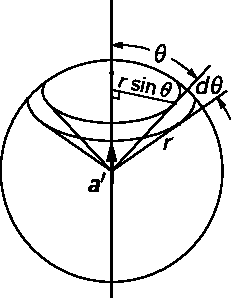
\includegraphics[width=0.7\linewidth]{fyz_fig267.pdf}
      \caption{Plocha kulového pásu je \(2\pi r\sin\vartheta\cdot r\dd{\vartheta}\) 
               (\cite[s.~427]{Feynman01})}
      \label{fyz:fig267}
    \end{figure}

    \begin{figure}[ht!] %\ref{fyz:fig268}
      \centering
      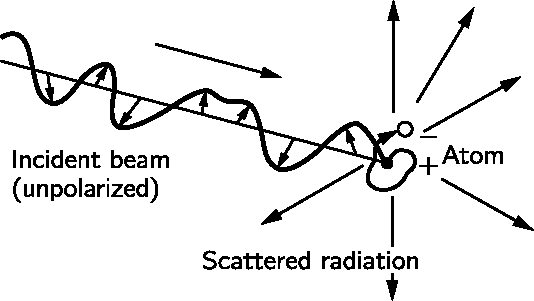
\includegraphics[width=0.9\linewidth]{fyz_fig268.pdf}
      \caption{Svazek záření dopadá na atom a uvádí do pohybu náboje (elektrony), které jsou v něm. 
               Pohybující se elektrony vzápětí vyzařují v různých směrech
               (\cite[s.~432]{Feynman01})}
      \label{fyz:fig268}
    \end{figure}

    \begin{figure}[ht!] %\ref{fyz:fig269}
      \centering
      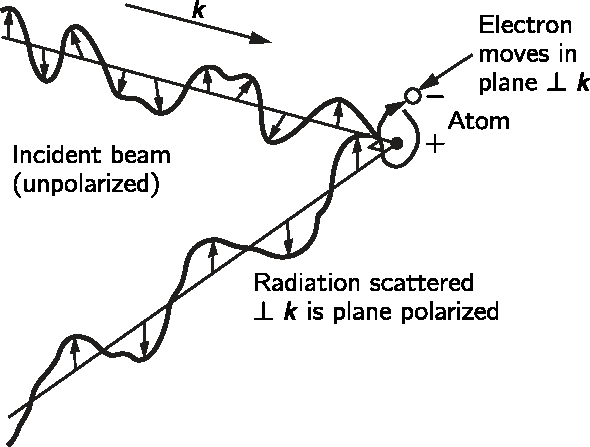
\includegraphics[width=0.9\linewidth]{fyz_fig269.pdf}
      \caption{Znázornění vzniku polarizace záření rozptýleného pod pravým úhlem k původnímu svazku
               (\cite[s.~435]{Feynman01})}
      \label{fyz:fig269}
    \end{figure}
    
} %tikzset
%---------------------------------------------------------------------------------------------------
\printbibliography[title={Seznam literatury}, heading=subbibliography]
\addcontentsline{toc}{section}{Seznam literatury}